

% [You should answer the question: What is the problem?]

% This paragraph should establish the context of the reported work. To do that, authors discuss over related literature (with citations\todo{How to make citations}\footnote{To cite a work in latex  }) and summarize the knowledge of the author in the investigated problem.

% An introduction should answer (most of) the following questions:
% \begin{itemize}
% 	\item What is the problem that I want to solve?
% 	\item Why is it a relevant question?
% 	\item What is known before the study?
% 	\item How can the study improve the current solutions?
% \end{itemize}

% To write it, use if possible active voice:
% \begin{itemize}
% 	\item I are going to watch a film tonight (Active voice).
% 	\item A film is going to be watched by us tonight (Passive voice).
% \end{itemize}
% The use of the first person is accepted.

\chapter{Introduction}
Since the development of robot technology in modern society, the robot's reliability and efficiency increase rapidly. Therefore, robots have been used together as a multi-robot system, which has advantages over single robots \cite{Eijyne2020DevelopmentOA}. Multi-robot systems are widely used in office environments to help people accomplish their goals. In addition to interacting with people, robots also need to learn from the surrounding environment to schedule their activities effectively. 

 For a working robot, environmental information is indispensable for efficiently perform activities. There are two types of environmental information. The first type is information about its surroundings, such as furniture, doors, walls, and other robots. The second type is the room occupation, which means the probability of someone in the office. In other words, in a typical office environment, people have different working schedules. If at least one person is in the office, the office is considered occupied. In this research, the knowledge of room occupancy is applied to task scheduling by the robot system. Finding a way to gather room occupancy information is a goal of this thesis. The robot can be equipped with external sensors and tools such as an infrared sensor, Laser Distance Sensor (LDS), and Camera. These modules can detect obstacles. However, compared with an office environment, the robot's perspective is limited, and the field within the sensing range is relatively narrow. To be more precise, robots cannot provide heterogeneous information relevant to infer room occupation over long periods. 

\section{Motivation}
This project's primary motivation is to improve the scheduling of tasks. 
Task scheduling determines when, where, and what order tasks need to be done by multiple robots. One of the most crucial research areas in multi-robot systems is the task scheduling problem. Task scheduling is an actual problem in many real-life applications, e.g., healthcare applications to assist elderly residents \cite{retire2017} inspection applications for industrial plants \cite{Chun12}. A report about the delivery robot in the hospital shows that a multi-robot system saves 2.8 full-time equivalent employees, as the robot works two shifts and seven days per week \cite{Jeon17}. 

It then becomes essential to improve task scheduling in office environments. Task scheduling can be improved in several aspects. The first aspect is to reduce the time required to complete a set of tasks. The second aspect is to minimize the energy consumption of the robots. The knowledge of room occupation can improve task scheduling in office environments. With knowledge of room occupation, robots can find people in the environment and avoid wasting time and energy in empty rooms \cite{retire2017}. However, it is almost impossible to sense all of the necessary information using only individual robots and sensors attached to it due to their limited perspective. 

Therefore, it is necessary to adopt the Internet of Things (IoT) devices in office environments \cite{PYO2015148}. Although increasing amounts of research have been conducted in task scheduling for multi-robot systems \cite{Shah7}, unfortunately, current research mainly focuses on multi-robot cooperation dynamic environments. Rarely research addresses applying the Internet of Things technologies in task scheduling because many people often think about the Internet of Things (IoT) and robotics technology as separate fields. One of the most critical research fields of IoT is the wireless sensor networks (WSN), which are easy to deploy and widely use in indoor environments \cite{Li8334565}.






\section{Problem definition}

Our problem concerns robots that must perform various tasks in office environments. The office environment should consist of multiple rooms. In this project, I assume no robot limitation in these rooms. As long as the door of the room is opened, any robot can enter it. The people can have their working schedules, which cause the room occupied and unoccupied regularly. I assume each room has one or multiple doors, and each door is attached to a sensor. I consider charging stations for robots because the robot energy level drops as it moves and rotates. 

If a set of different navigation tasks randomly distributed in different rooms. The system should be able to schedule these tasks. The navigation task requires one robot to traverse a path in the office environment. Particularly, a navigation task can have one or multiple target positions. In other words, the robot can navigate to a destination or pass through several positions and finally reach the destination. An efficient centralized task scheduling algorithm should be implemented for the multi-robot system using room occupation knowledge.

Besides performing navigation tasks, robots should also gather room occupation information from the office environment. Robots should gather room occupation information while performing tasks. The system should be able to share the information among sensors, robots, and the central pool. The centralized pool is the global controller that receives information about the robots and the environment and make decisions base on the information. Also, the robots with low-energy should go to a nearby charging station so that it has sufficient power to keep performing tasks.
An example of office environment is shown in Figure \ref{fig:example_environment}.

\begin{figure}[htbp]
    \centering
    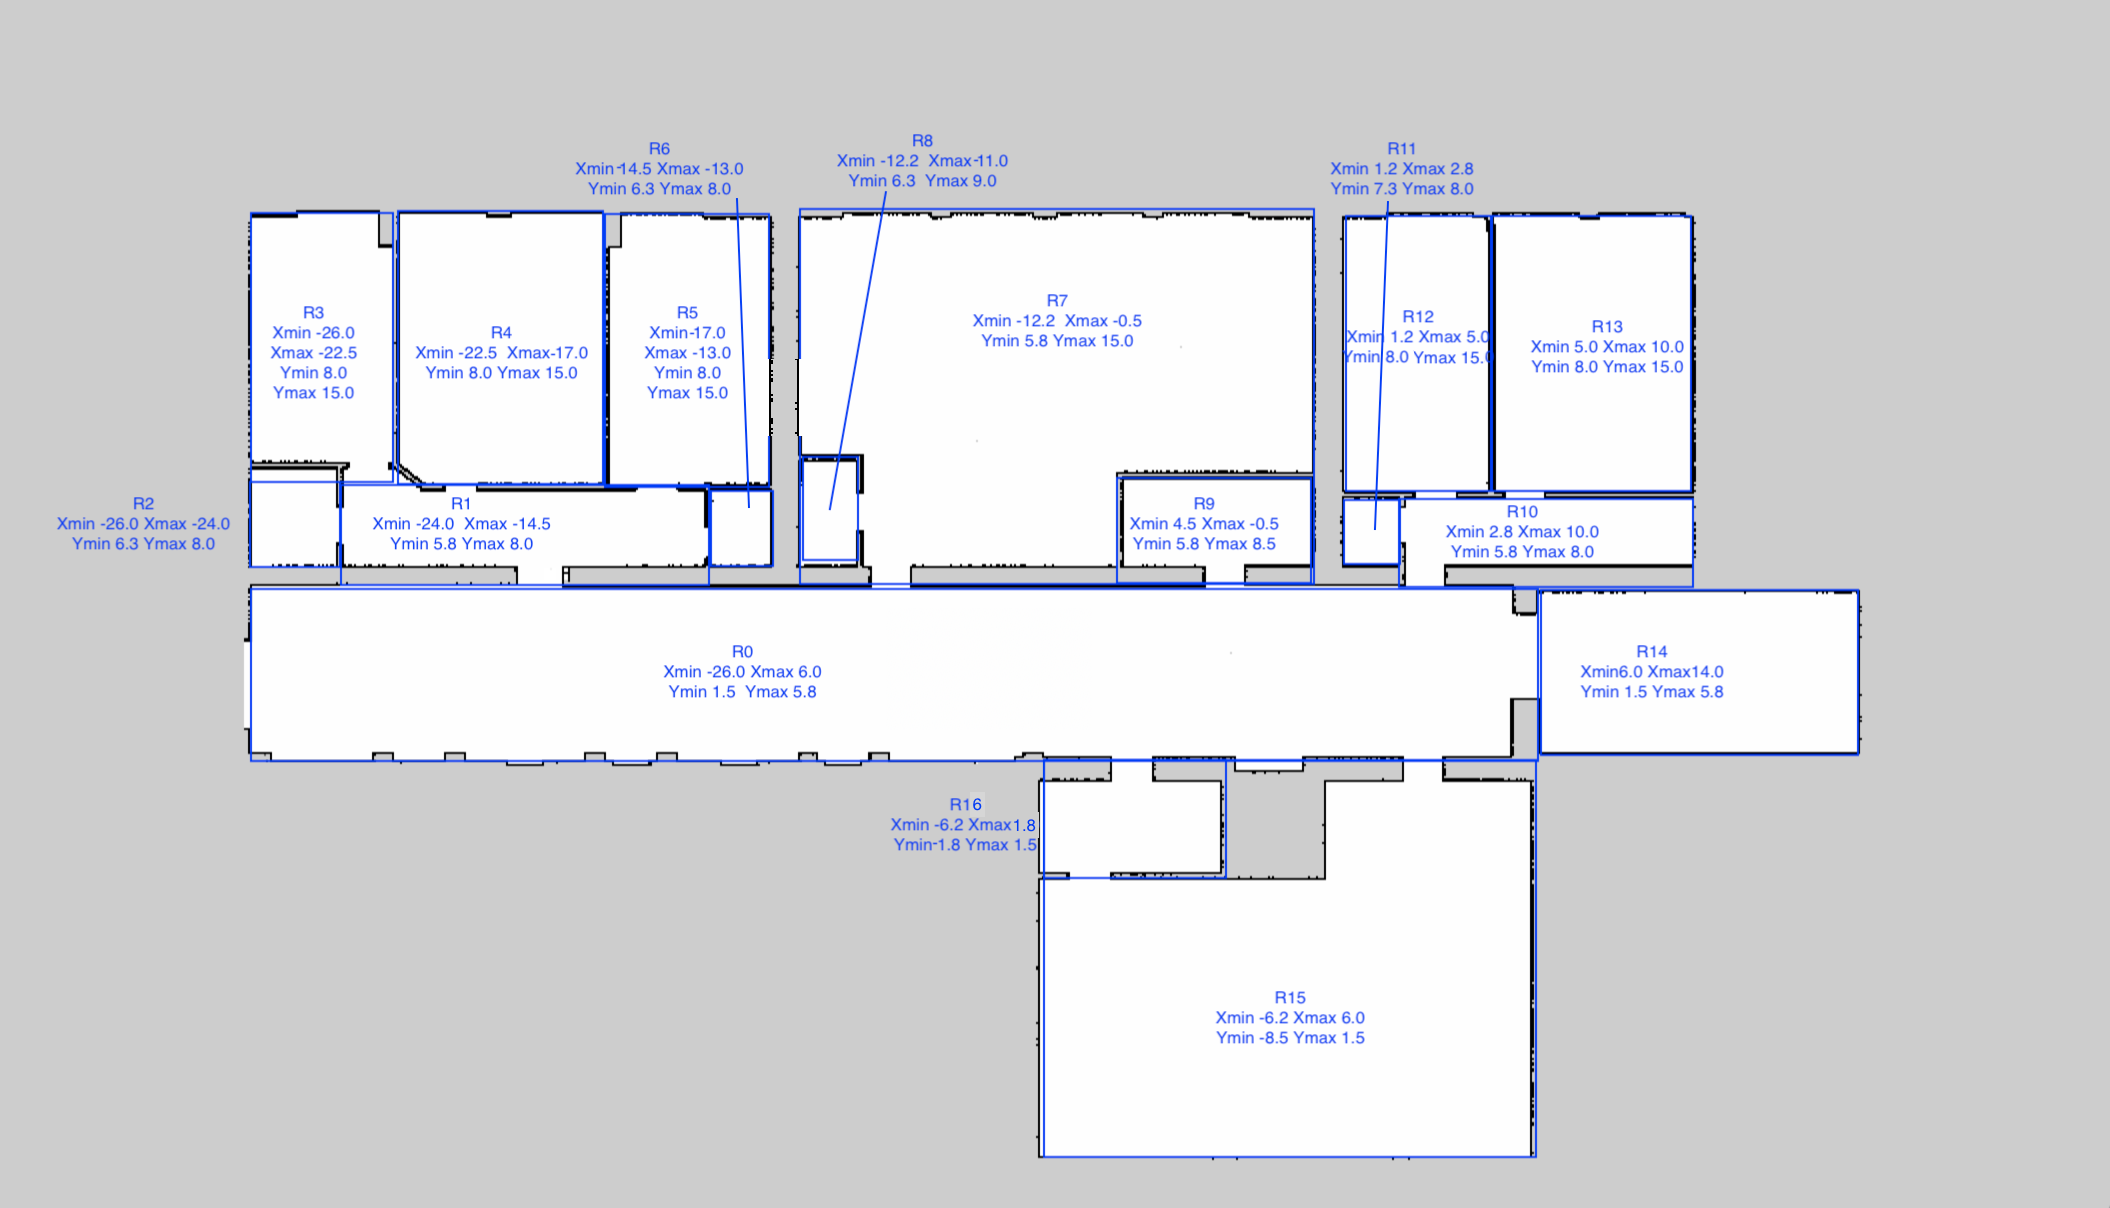
\includegraphics[width = 0.7\textwidth]{content/images/ch1/room_division.png}
    \caption{An example of office environment. There are 16 Rooms in this office environment.}
    \label{fig:example_environment}
\end{figure}

\section{Main Contributtions}

I have designed a method for robots to gather room occupation information while performing tasks. As long as the robot enters the sensor range, they conduct a rapid exchange of room occupation information. The robot then sends acquired room occupation data to the centralized pool. The centralized pool is the global controller that receives information about the robots and the environment and make decisions base on the information. The centralized pool uses this information in two ways. It assigns robots the navigation tasks according to the information and can assign robots to explore the room lacking the information. Once the robot finished current tasks, it notifies the central pool that the task is succeeded and requests a task from the centralized pool.

I also have implemented a multi-robot task scheduling method in the centralized pool. The goal of multi-robot task scheduling is to decrease the time of completion and energy consumption. Moreover, the centralized pool can use room occupation information as one evaluation parameter to schedule tasks, together with common evaluation parameters such as priority, waiting time, energy consumption, etc. Task priority means the importance of tasks. The waiting time is the difference between the current time and task start time. Energy consumption is the amount of energy expected to be reduced by performing a task.

I also paid attention to increasing the number of tasks complete. When a robot cannot perform its current task, it hands over tasks to other robots. To be more precise, sometimes, the robot can not perform the current task within a fixed deadline since the target position is temporarily unreachable (e.g., blocked by a closed-door). In this case, the blocked robot sends failure detail to the centralized pool and request another task. The failed task will then be reused for task scheduling. 


In addition to the architecture I proposed herein, our system uses the Robot Operating System (ROS) platform to archive core autonomous robot function (navigation, localization, and mapping). Thanks to the ROS, I was able to develop a flexible and efficient system. Adding or removing modules, including robots, sensors, or charging stations, is simple and straightforward.

\section{Thesis Structure}

The next chapter briefly introduces background information. The essential concept about the Robot Operating System (ROS) and ROS Tools are introduced, along with a discussion of previous task scheduling methods.

Chapter 3 formally presents the architecture of the multi-robot system and gives information about tasks. The approaches to schedule tasks are also introduced.

Chapter 4 focuses on the implementation of each component in the multi-robot system. It presents the way robots gather room occupation information while performing tasks. 

Chapter 5 introduces the approach to the evaluation, along with the simulated office environment. It also demonstrates the simulation results acquired using the approach. Besides, a quantitative experiment analysis was performed.

Finally, chapter 6 discussed the results of the performed work and future work. The impact of limitations of simulation on the experimental results is also discussed.






